\documentclass[a4paper, 11pt]{article}

\usepackage{graphicx}
\graphicspath{ {/media/data/Documents/Panepisthmio/} {img/}}
\usepackage{tabularx}
\usepackage{hyperref}
\usepackage{listings}
\usepackage{xcolor}

\begin{document}

\begin{center}
\section*{System Analysis}
\end{center}

\begin{figure}[h]
  \centering
  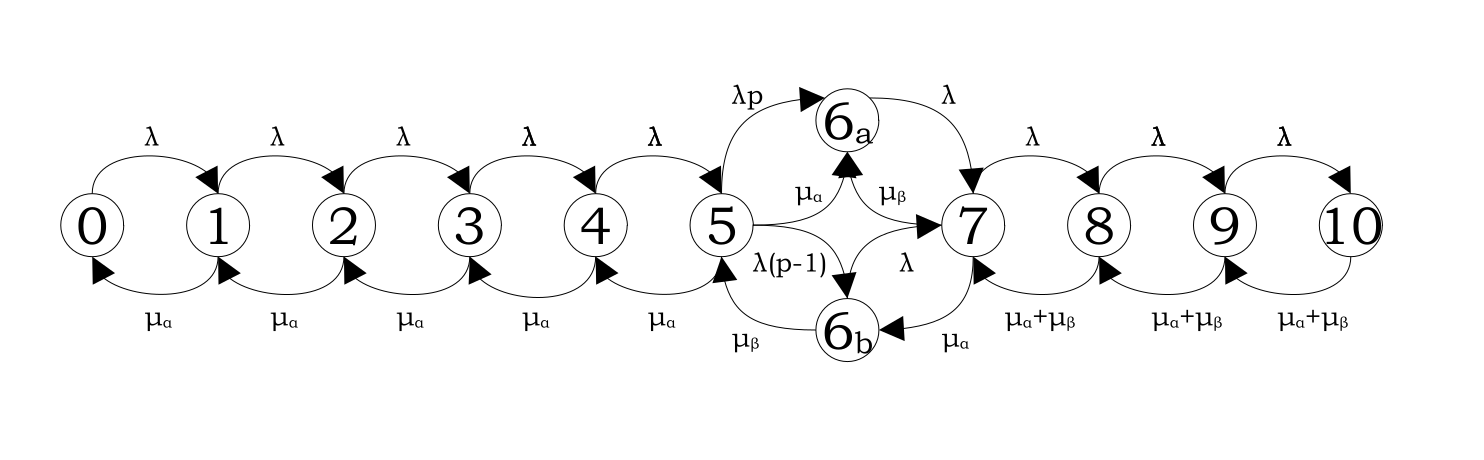
\includegraphics[trim = 140 0 0 0, width = 14cm, keepaspectratio]{states.jpg}
  \caption{Diagram of Transitions}
\end{figure}

\paragraph{} From Local Balance Equations:
\begin{displaymath}
  \lambda P_0 = \mu_\alpha P_1 \Leftrightarrow P_1 = \frac{\lambda}{\mu_\alpha} P_0
\end{displaymath}

\begin{displaymath}
  \lambda P_1 = \mu_\alpha P_2 \Leftrightarrow P_2 = {\left(\frac{\lambda}{\mu_\alpha}\right)}^2 P_0
\end{displaymath}

In general:
\begin{equation}\label{pi5}
  P_i = {\left(\frac{\lambda}{\mu_\alpha}\right)}^i P_0,\quad i = 1, 2, 3, 4, 5
\end{equation}

\paragraph{} For the states $6_a$ and $6_b$, a general state 6 is defined,
where $P_6 = P_{6a} + P_{6b}$.

\begin{displaymath}
  \lambda P_5 = (\mu_\alpha + \mu_\beta)P_6 \Leftrightarrow
  P_6 = {\left(\frac{\lambda}{\mu_a + \mu_b}\right)} P_5 \Leftrightarrow
\end{displaymath}
\begin{equation}\label{p6}
  \Leftrightarrow P_6 = \frac{\lambda}{\mu_a + \mu_b} {\left(\frac{\lambda}{\mu_a}\right)}^5P_0
\end{equation}

\begin{displaymath}
  2\lambda P_6 = (\mu_\alpha + \mu_\beta)P_7 \Leftrightarrow
  P_7 = {\left(\frac{2\lambda}{\mu_a + \mu_b}\right)P_6} \Leftrightarrow
  P_7 = 2{\left(\frac{\lambda}{\mu_a + \mu_b}\right)}^2 {\left(\frac{\lambda}{\mu_a}\right)}^5P_0
\end{displaymath}

In general:

\begin{equation}\label{pi10}
  P_i = 2 {\left(\frac{\lambda}{\mu_a + \mu_b}\right)}^{i-5}
  {\left(\frac{\lambda}{\mu_a}\right)}^5 P_0,\quad i = 7, 8, 9, 10
\end{equation}

\paragraph{} From normalisation and~\ref{pi5},~\ref{p6},~\ref{pi10},:

\begin{displaymath}
  \sum_{i=0}^{10} P_i = 1 \Leftrightarrow
\end{displaymath}
\begin{displaymath}
  P_0 = {\left[
  1 + \frac{\lambda}{\mu_a} + {\left(\frac{\lambda}{\mu_a}\right)}^2 +
  \cdots +
  \frac{\lambda}{\mu_a + \mu_b}{\left(\frac{\lambda}{\mu_a}\right)}^5 +
  2{\left(\frac{\lambda}{\mu_a + \mu_b}\right)}^2 {\left(\frac{\lambda}{\mu_a}\right)}^5 +
  \cdots
  \right]}^{-1}
\end{displaymath}

\paragraph{} The mean number of clients is derived from the formula:

\begin{displaymath}
  E[n(t)] = \sum_{i=0}^{10} iP_i =
\end{displaymath}

\begin{displaymath}
  = {\left[
      \frac{\lambda}{\mu_a} +
      2 {\left(\frac{\lambda}{\mu_a}\right)}^2 +
      \cdots +
      6 \frac{\lambda}{\mu_a + \mu_b} {\left(\frac{\lambda}{\mu_a}\right)}^5 +
      7 \times 2 {\left(\frac{\lambda}{\mu_a + \mu_b}\right)}^2 {\left(\frac{\lambda}{\mu_a}\right)}^5 +
      \cdots
  \right]} P_0
\end{displaymath}

Finally, throughput is calculated from the formula:

\begin{displaymath}
  \gamma = \lambda(1 - P_{blocking}) = \lambda(1 - P_{10})
\end{displaymath}


\end{document}
